\section{Sample Production}
\label{sec:sample_production}

The sample production science unit is focused on validating and verifying a number of later stage data products. 
As such, this science unit has been slow to ramp up but is engaging as we process more ComCam data through the DRP. 

Some of the early highlights include running synthetic source injection of stars and galaxies to measure catalog completness and reliability. 
Figure \ref{fig:ssi_comp} shows an example figure showing i-band completness and purity as a function of magnitude for ECDFS (tract=5603).
\begin{figure}
    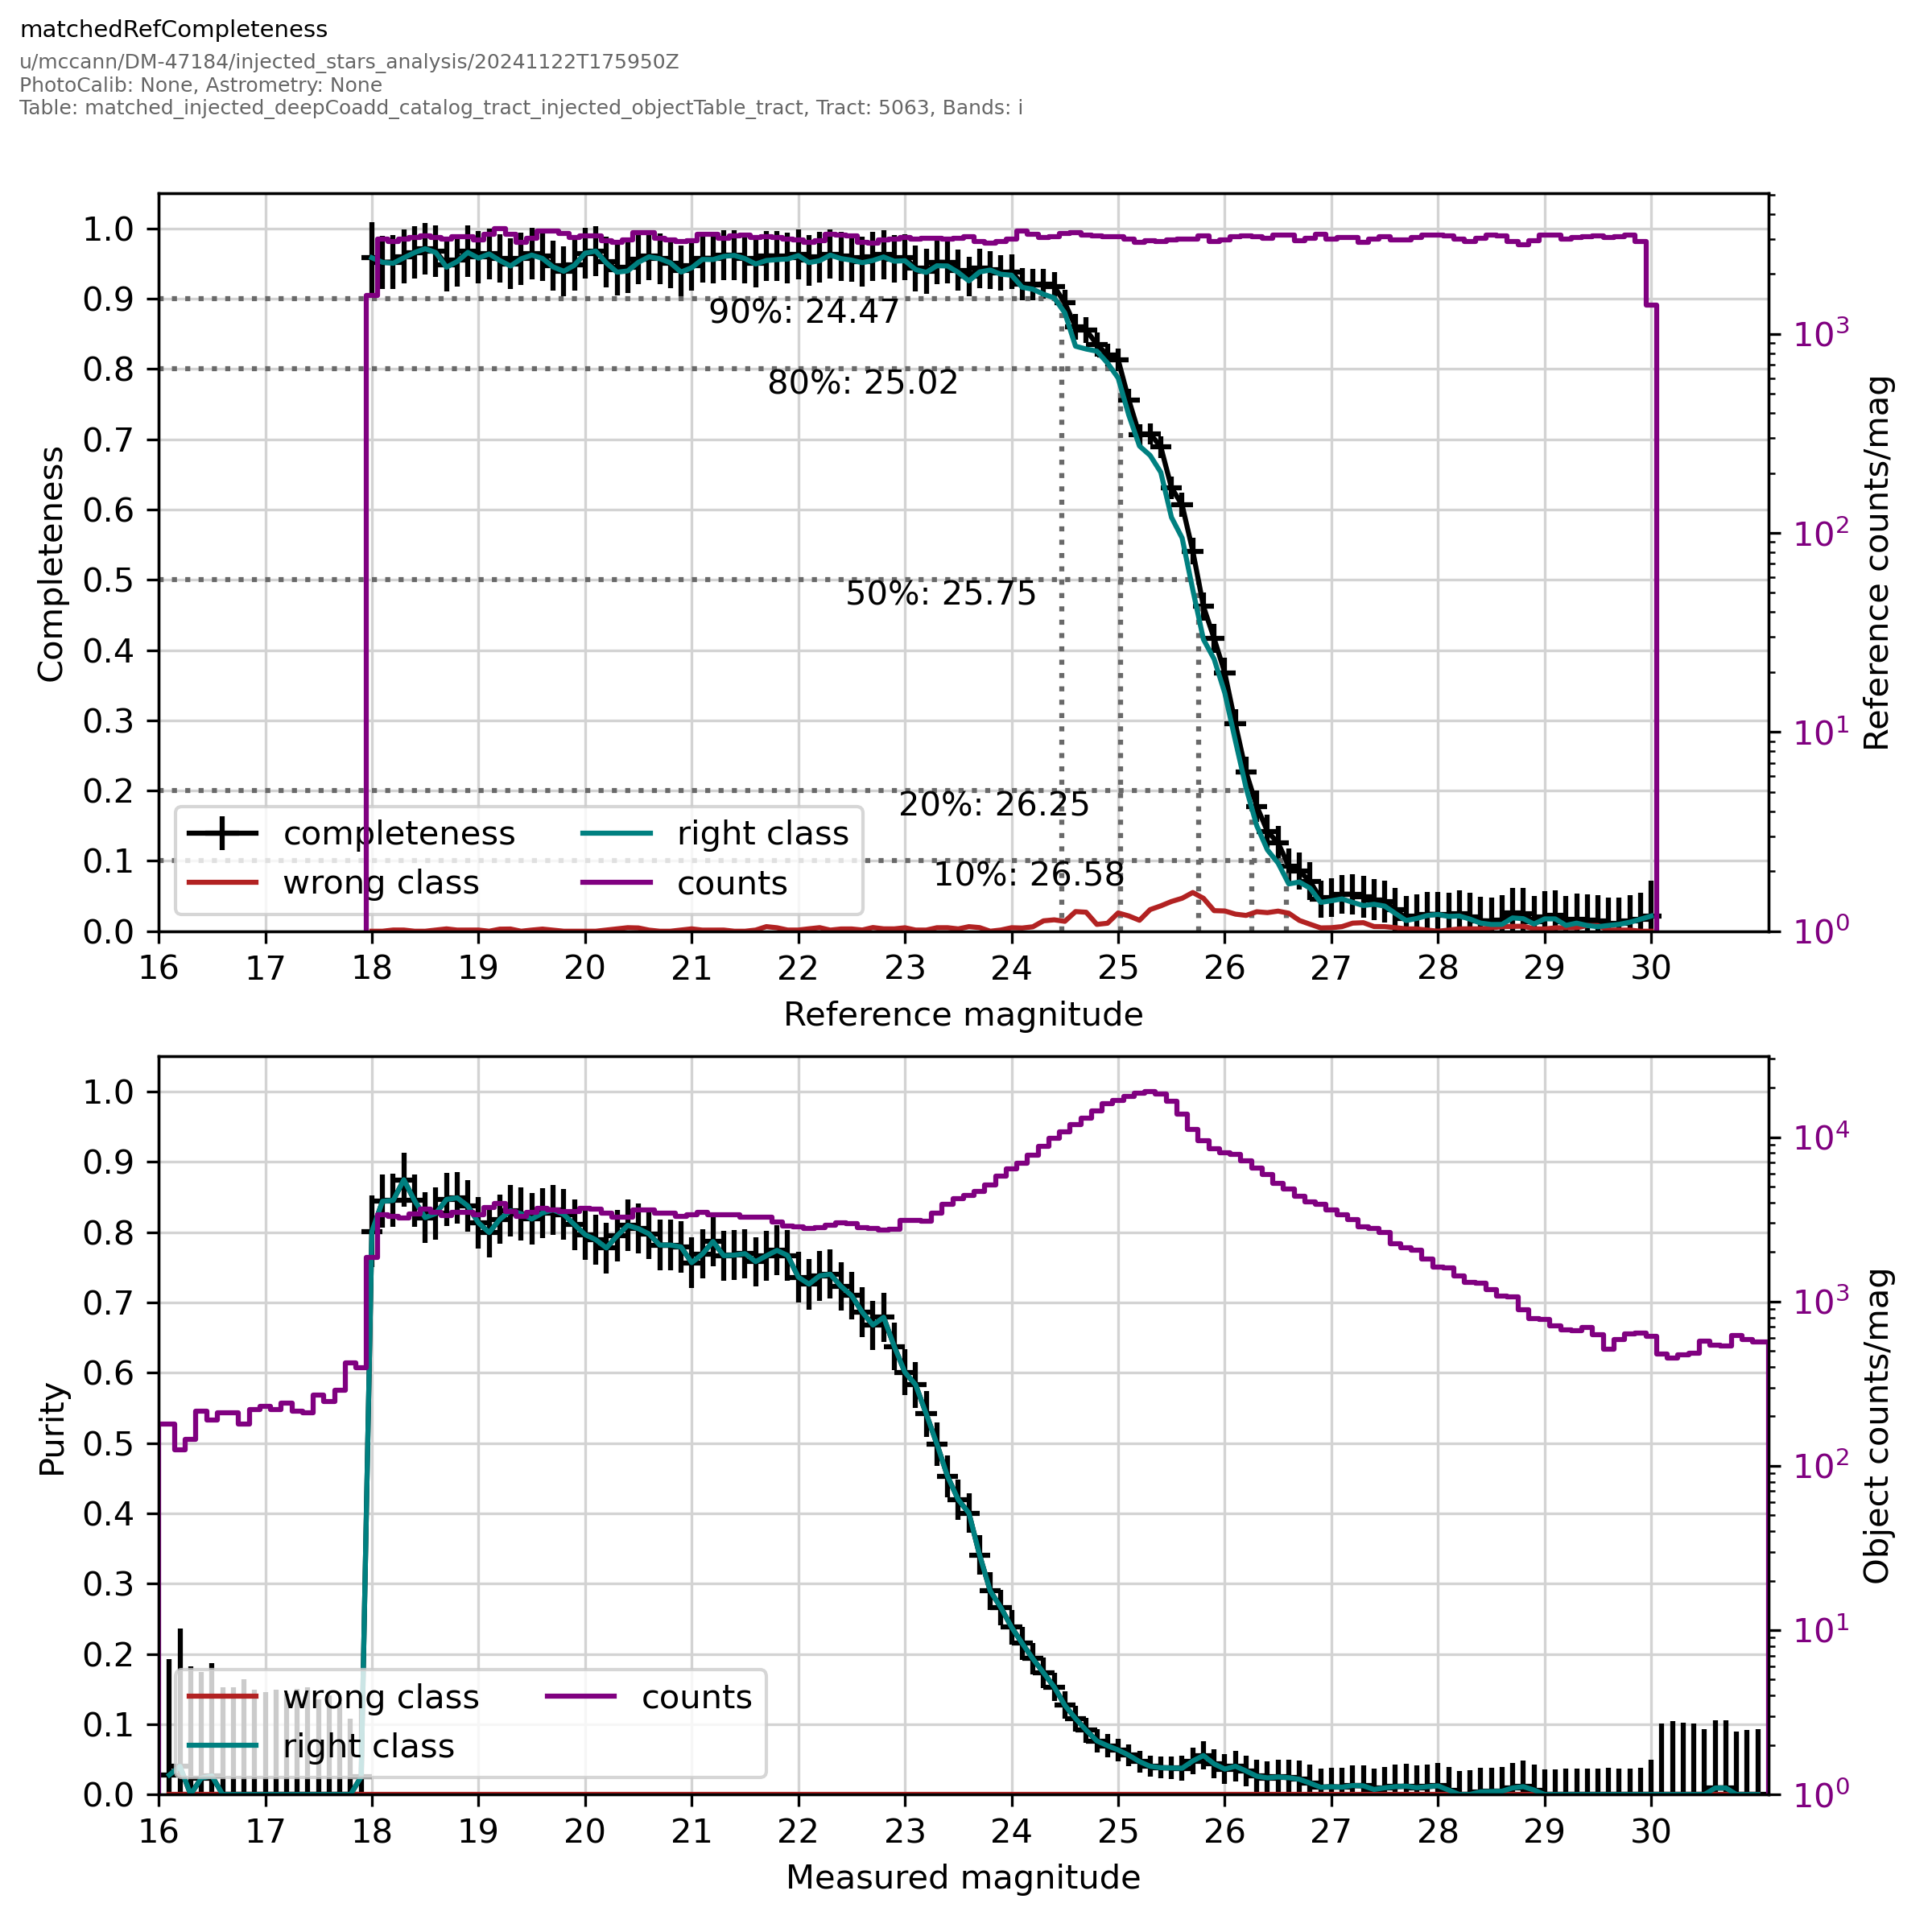
\includegraphics{sample_production_figures/matched_ref_completness_ssi_i.png}
    \caption{SSI based measurements of completeness and purity in the i-band.}
    \label{fig:ssi_comp}
\end{figure}

We also confirmed a strategy to use twilight observations to verify the system can accurately observe bright starts (1 mag brighter than 15 saturation lim). 

  
  